\documentclass[review]{elsarticle}
\usepackage{hyperref}
\usepackage[margin=1in]{geometry}
\usepackage{graphicx}
\usepackage{amsmath}
\usepackage{placeins}
\usepackage{comment}
\usepackage{gensymb}
\usepackage{lineno}


\journal{Journal of Nuclear Materials}
\bibliographystyle{elsarticle-num}

\begin{document}

\begin{frontmatter}
\title{An atomistic study of grain boundaries and surfaces in $\gamma$U-Mo}

\author[inl]{Benjamin Beeler\corref{qwe}}
\cortext[qwe]{Corresponding author}
\ead{benjamin.beeler@inl.gov}
\author[inl]{Yongfeng Zhang}
\author[inl]{Yipeng Gao}
\address[inl]{Idaho National Laboratory, Idaho Falls, ID 83415}


\begin{abstract}
A monolithic fuel design based on a U-Mo alloy has been selected as the fuel type for conversion of the United States High-Performance Research Reactors (HPRRs). A 2015 post-irradiation examination (PIE) report showed accelerated swelling in U-10Mo fuels at fission densities much lower than previously observed. This PIE report showed a large amount of compositional banding, or regions of low Mo content adjacent to regions of high Mo content, with low Mo content typically along grain boundaries. Lower Mo content can lead to phase decomposition from the gamma U-Mo body-centered cubic phase to the alpha U phase as well as an earlier onset of recrystallization. Thus, the phenomenon of Mo depletion at grain boundaries is an important factor in the accelerated swelling behavior of U-Mo fuel. However, the physical origin of Mo depletion at grain boundaries is still unclear. In this work, molecular dynamics simulations have been performed to calculate the grain boundary and surface energies of body-centered cubic (bcc) U, bcc Mo and alloys of U-Mo from 600 K to 1200 K. It is observed that the lower grain boundary energy of bcc U, compared to bcc Mo, provides the driving force for Mo depletion at grain boundaries. This driving force diminishes with increasing temperature, but is not eliminated. This information can be utilized as inputs to higher length scale modeling methodologies and provide specification guidance to fabricators.
\end{abstract}
\end{frontmatter}

\linenumbers
\modulolinenumbers[5]

\section{Introduction}

There has been a renewed effort in recent decades to replace current highly enriched uranium (HEU) fuel in high power research reactors with low enriched uranium (LEU) fuel \cite{snelgrove1997}. In the United States, this program is the United States High-Performance Research Reactor (USHPRR) program. Research reactors require fuel that operates at high power and reaches high fission density, but at relatively low temperatures. As such, UO$_{2}$ fuel utilized in commercial nuclear reactors is non-viable for research reactor use. Typical research reactor fuel consists of aluminum (Al) cladding surrounding a fuel meat composed of fuel particles dispersed in an Al matrix \cite{meyer2014}. In order to achieve a reduced enrichment in these fuel types, there is the requirement for increased uranium density. One way this is achieved is by utilizing $\gamma$ stabilized uranium alloys with 10 wt.\% or less alloy content. The fuel design being pursued under the USHPRR program is a uranium-molybdenum (U-Mo) monolithic foil, with a zirconium (Zr) diffusion barrier in Al clad, as shown in Fig. \ref{fig:ben1}. 

\begin{figure}[!h]
 \centering
 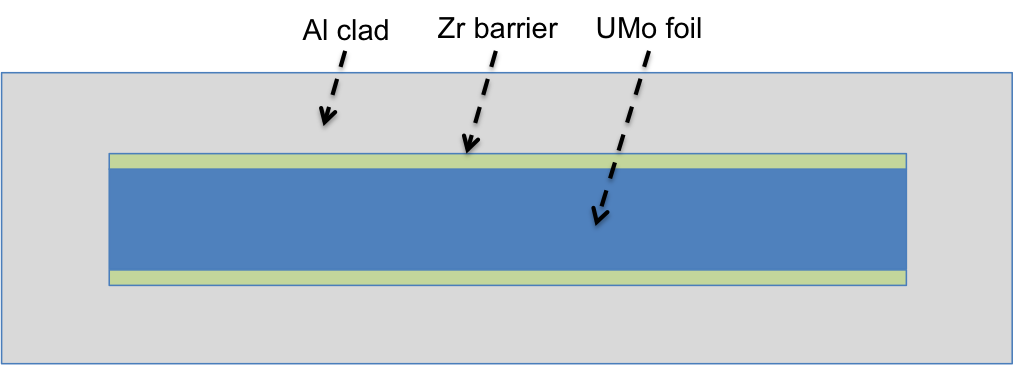
\includegraphics[width=0.8\textwidth]{ben1.png} 
 \caption{Schematic of U-Mo monolithic fuel cross section. Not to scale.}
 \label{fig:ben1}
\end{figure}

\FloatBarrier

One issue with metallic fuels, including U-Mo, is the large amount of swelling that takes place during operation\cite{hofman1997}. Such swelling can be accounted for in the fuel design, however the swelling needs to be stable and predictable up to high fission densities. Research reactor fuel types based on U-Mo are unique in their ability to stably retain fission gases to high fission densities, and as such there is a relatively high content of fission gas and of fission gas bubbles within the fuel matrix. The importance of swelling in addition to the unique fuel environment has led to a variety of studies attempting to characterize the swelling behavior in U-Mo fuels \cite{rest2009, kim_anl08, meyer2002, kim2013} which has led to the development of a swelling correlation as a function of fission density from Argonne National Labortory (ANL correlation) \cite{kim2011} and Idaho National Laboratory \cite{umo_prelim_report2017}. The ANL correlation was intended to be applicable for low temperature (less than 250$^{\circ}$C) U-Mo alloys in the 7-10 wt.\% composition range. 

A 2015 post-irradiation examination (PIE) report \cite{afip6report} from Williams, et al. showed higher swelling in U-10Mo fuels at fission densities much lower than previously observed. This accelerated fuel swelling behavior could lead to early fuel failure and was not captured by the ANL correlation. Understanding the cause of this anomalous swelling behavior is a critical step in qualifying U-Mo fuel for use in research reactors. This PIE report showed a large amount of compositional banding, or regions of low Mo content adjacent to regions of higher Mo content, with low Mo content typically along grain boundaries. An increased amount of swelling was also observed in lower Mo content alloys (U-7Mo) \cite{vandenberghe2014} at lower fission densities. Lower Mo content can lead to phase decomposition from the $\gamma$U-Mo body-centered cubic (bcc) phase to the face-centered orthorhombic $\alpha$U phase \cite{janfong2014}. This is evident along grain boundaries as well as in the region involving the interaction of the U-Mo fuel foil and the Zr diffusion barrier \cite{park2015}. Finally, in alloys with either lower Mo content or increased banding, it has been observed an earlier onset of irradiation-induced recrystallization\cite{kim2013A}, where new nano-sized grains are being formed primarily along grain boundaries. Recrystallization is the suggested culprit behind accelerated swelling, as the recrystallized grains are destroying the fission gas superlattice \cite{vandenberghe2008}. 

This experimental history suggests that the phenomenon of Mo depletion at grain boundaries is an important factor in the accelerated swelling behavior of U-Mo fuel. In order to understand this phenomenon, we need to discover the driving force explaining why it occurs. This driving force must then be studied to determine its variance as a function of a variety of properties in order to determine if there is a way to diminish the driving force behind Mo depletion, aiding in the fuel fabrication processes, with the goal of improving the swelling behavior of U-Mo fuel.

Previous computational investigations have been performed investigating grain boundary energies in bcc Mo by Morita \cite{morita1997} and Wolf \cite{wolf1989bcc1, wolf1990bcc2} utilizing a Finnis-Sinclair potential \cite{finnis}. Yesilleten and Arias \cite{yesilleten2001} utilized a model generalized pseudopotential theory (MGPT) \cite{moriarty1988} potential to investigate bcc Mo grain boundaries and their interactions with vacancies. Ratanaphan \cite{ratanaphan2015} also utilized the Finnis-Sinclair potential \cite{finnis} to comprehensively study Mo grain boundaries within a molecular statics framework. Novoselov \cite{novoselov2014} studied the interactions of vacancies and interstitials with grain boundaries in bcc Mo using an Embedded-Atom Method (EAM) \cite{daw1984, daw1993} potential \cite{starikov2011}. A recent first principles study investigated surface energies in U-Mo \cite{zhigang2018}. To the best of our knowledge, in the literature there are not any high temperature computational studies on bcc Mo grain boundaries nor any computational studies whatsoever of bcc U or U-Mo alloy grain boundaries.

In this paper, molecular dynamics simulations have been performed to calculate the grain boundary and surface energies of bcc U, bcc Mo and alloys of bcc U-Mo from 600 K to 1200 K. 

\section{Computational Details}
\subsection{Interfacial energy calculations}
Molecular dynamics simulations are performed utilizing the LAMMPS \cite{plimpton1995} software package and the U-Mo angular dependent potential (ADP) \cite{smirnovaADP}. A supercell with periodic boundaries is generated that contains two grain boundaries or two free surfaces. The size of the supercell depends on the nature of the interfaces (grain boundaries/surfaces) investigated. Eleven grain boundaries (ten symmetric and one asymmetric) are constructed with respect to the $\langle$100$\rangle$ tilt axis. The asymmetric tilt grain boundary is constructed by only tilting half of the supercell, while holding the rest of the supercell fixed. Grain boundary system size is dependent upon the interface orientation, ranging from between 3000 and 6500 atoms. Three unit cells are included along the tilt axis. Seven unique surfaces are investigated, including three high symmetry surfaces and four lower symmetry surfaces. The low symmetry surfaces are constructed in the same manner as grain boundaries, however only half of the system is constructed as to generate two surfaces instead of two grain boundaries. An example system for the U-10Mo \{120\} symmetric tilt grain boundary is shown in Fig. \ref{fig:gbex} (U-10Mo refers to 10 weight percent Mo, approximately 22 atomic percent).

\begin{figure}[h]
 \centering
 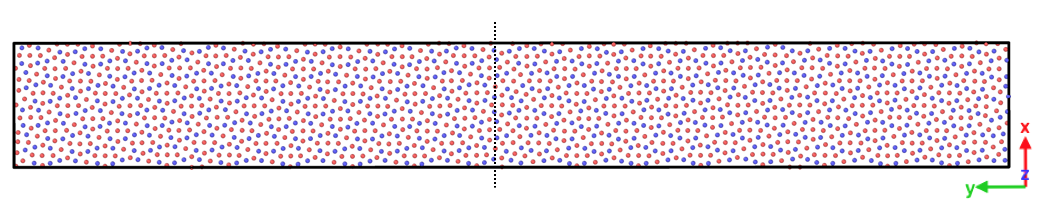
\includegraphics[width=0.8\textwidth]{gbex.png} 
 \caption{The U-10Mo \{120\} symmetric tilt grain boundary at 600 K. Grain boundaries exist in the middle and on the edges of the supercell. Red atoms are uranium and blue atoms are molybdenum.}
 \label{fig:gbex}
\end{figure}

These systems were verified to be large enough to obtain accurate surface energies by investigating a single representative larger system and comparing respective interfacial energies. Relaxation is performed in an NPT-ensemble, relaxing each x, y, and z component individually, with a damping parameter of 0.1. A Langevin thermostat in the Gronbech-Jensen-Farago \cite{gjf2014} formalism is utilized with the damping parameter set to 0.01 ps. Systems are relaxed for 100 ps, with energies averaged over the final 50 ps. Five unique simulations are performed for each system to ensure statistical significance of the results. The interfacial energy is calculated via equation \ref{eq:surface},

\begin{equation}
\label{eq:surface}
E_{nf}= \frac{(E^{*} - E)}{A} \times N
\end{equation}

where $\it{E^{*}}$ is the energy per atom of the system with two interfaces, $\it{E}$ is the energy per atom of the perfect crystal U, Mo or U-Mo, $\it{A}$ is the total area of the interface (there are two in the system) and $\textit{N}$ is the number of atoms in the system with two interfaces. 

Alloys of U-Mo are generated by constructing a bcc U grain boundary system, with a prescribed number of U atoms replaced by Mo. Thus, both the bulk and the grain boundary should be of the same alloy concentration. Unique systems are developed for each interfacial configuration by generating five different U-Mo configurations at the prescribed alloy concentrations. For pure U and pure Mo, unique systems are developed by initializing velocities with different random number seeds. 

\subsection{Mo depletion at interfaces}

In order to investigate potential depletion of Mo at grain boundaries, a hybrid Monte Carlo/Molecular Dynamics (MC/MD) methodology is employed. A \{120\} symmetric tilt grain boundary with a U-10Mo concentration is constructed and a series of atom swaps are performed via the atom/swap function within LAMMPS. This function performs Monte Carlo swaps of atoms of one given atom type with atoms of a second given atom type \cite{plimpton1995}, maintaining a fixed global concentration. Atoms of U and Mo are swapped at every other timestep while the system is simultaneously equilibrated in an NPT ensemble, resulting in a hybrid MC/MD simulation. If the potential energy of the system is reduced via the atomic swap, then the swap is accepted. If the potential energy is increased via the swap, there is a probability of accepting the swap based on a specified scaling temperature, set at 1000 K within these simulations. The swap simulation is performed for 500,000 timesteps and thus 250,000 attempted swaps. This is sufficiently long to reach an equilibrium state, as the energy of the system is being reduced by less than 2$\times$10$^{-3}$ eV/at over the final 100,000 timesteps.

\section{Results}
\subsection{BCC Mo Interfacial Energies}

\subsubsection{BCC Mo Grain Boundary Energies}

The bcc Mo grain boundary energy at 600 K as a function of misorientation angle with respect to the $\langle$100$\rangle$ tilt axis is shown in Fig. \ref{fig:mo600}. Results are compared to work from Morita \cite{morita1997} on bcc Mo utilizing a Finnis-Sinclair \cite{finnis} potential. Data from Morita \cite{morita1997} was extracted via WebPlotDigitizer \cite{webplot} and replotted alongside this work in Fig. \ref{fig:mo600}. Grain boundary planes studied within this work are labeled. Data points are connected with straight lines as a means to guide the eye. Qualitatively, the results from this work compare very favorably to the results from Morita. The most prominent minima observed are at the \{130\} and \{120\} grain boundary planes, whereas maxima are observed at the \{370\} and \{350\} planes. Generally, grain boundary energies are slightly lower than those predicted from Morita. It should be noted that the work from Morita was conducted at 0 K, whereas this work is at a non-zero temperature. 

\begin{figure}[h]
 \centering
 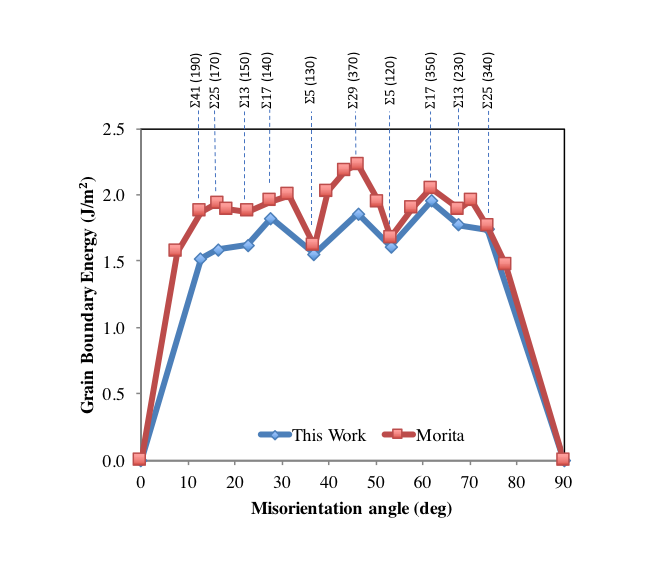
\includegraphics[width=0.6\textwidth]{mo600B.png} 
 \caption{The bcc Mo grain boundary energy as a function of misorientation angle with respect to the $\langle$100$\rangle$ tilt axis at 600 K. Results are compared to Morita \cite{morita1997}.}
 \label{fig:mo600}
\end{figure}

\FloatBarrier

The data from Fig. \ref{fig:mo600} is displayed in Table \ref{tab:mo600}, listing the ten unique symmetric tilt grain boundaries that were investigated for the bcc Mo system. The average standard deviation for each of these data points is 0.01 J/m$^{2}$. Excluding the low angle grain boundary of \{190\}, the minimum energy grain boundary plane examined is the \{130\}. The maximum energy grain boundary plane examined is the \{350\}, with a difference between the maximum and minimum of 0.40 J/m$^{2}$.

\begin{table}[h]
\caption{The bcc Mo grain boundary energy at 600 K for ten unique symmetric tilt grain boundaries. Grain boundary plane is with respect to the $\langle$100$\rangle$ tilt axis.} \label{tab:mo600}
\begin{center}
\begin{tabular}{|c|c|}
	\hline
	Grain Boundary Plane & Energy (J/m$^{2}$) \\
	 \hline
	 \{190\} & 1.52 \\
	 \{170\} & 1.59 \\
	 \{150\} & 1.62 \\
	 \{140\} & 1.82 \\
	 \{130\} & 1.55 \\	 
	 \{370\} & 1.85 \\
	 \{120\} & 1.61 \\
	 \{350\} & 1.95 \\
	 \{230\} & 1.77 \\
	 \{340\} & 1.74 \\
	 \hline
\end{tabular}
\end{center}
\label{default}
\end{table}

\FloatBarrier

The bcc Mo grain boundary energy as a function of temperature for four symmetric tilt grain boundaries and one asymmetric tilt grain boundary is shown in Fig. \ref{fig:motemp}. It can be observed that minimal variance is observed with increasing temperature for each respective grain boundary plane. However, there is a slight trend towards increasing grain boundary energy as a function of increasing temperature. The associated data is presented in Table \ref{tab:motemp}. Over the given temperature range, grain boundary energies only vary by a maximum of 0.05 J/m$^{2}$.

\begin{figure}[h]
 \centering
 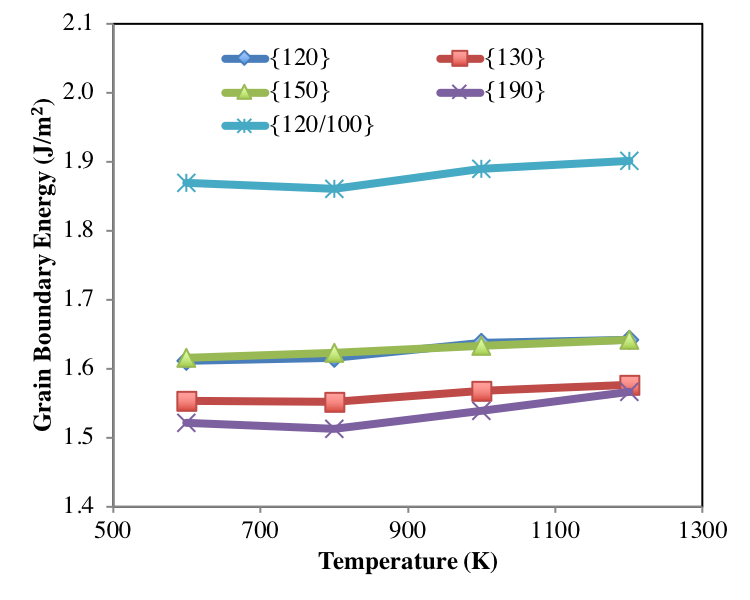
\includegraphics[width=0.6\textwidth]{mo_temp.png}
 \caption{The bcc Mo grain boundary energy as a function of temperature for five unique grain boundaries.}
 \label{fig:motemp}
\end{figure}

\FloatBarrier

\begin{table}[h]
\caption{The bcc Mo grain boundary energy from 600 K to 1200 K for five unique grain boundaries. Units in J/m$^{2}$. } \label{tab:motemp}
\begin{center}
\begin{tabular}{|c|c|c|c|c|}
	\hline
	Grain Boundary Plane & 600 K & 800 K & 1000 K & 1200 K \\
	 \hline
	 \{120\} & 1.61 & 1.62 & 1.64 & 1.64 \\
	 \{130\} & 1.55 & 1.55 & 1.57 & 1.58 \\
	 \{150\} & 1.62 & 1.62 & 1.63 & 1.64 \\
	 \{190\} & 1.52 & 1.51 & 1.54 & 1.57 \\
	 \{120/100\} & 1.87 & 1.86 & 1.89 & 1.90 \\	 
	 \hline
\end{tabular}
\end{center}
\label{default}
\end{table}

\FloatBarrier

\subsubsection{BCC Mo Surface Energies}

The bcc Mo surface energy for seven unique surfaces as a function of temperature is shown in Fig. \ref{fig:mosurf} and the associated data is presented in Table \ref{tab:mosurf}. It is observed that the \{110\} surface is the lowest energy surface in bcc Mo. This makes intuitive sense, as this is also the most closed-packed plane in the bcc crystal structure. The highest energy surface studied is the \{111\}. The surface energy shows a minor increase as a function of increasing temperature, similar to the trends of grain boundary energy as a function of temperature in Fig. \ref{fig:motemp}. Over the given temperature range, surface energies vary by a maximum of 0.14 J/m$^{2}$.

\begin{figure}[h]
 \centering
 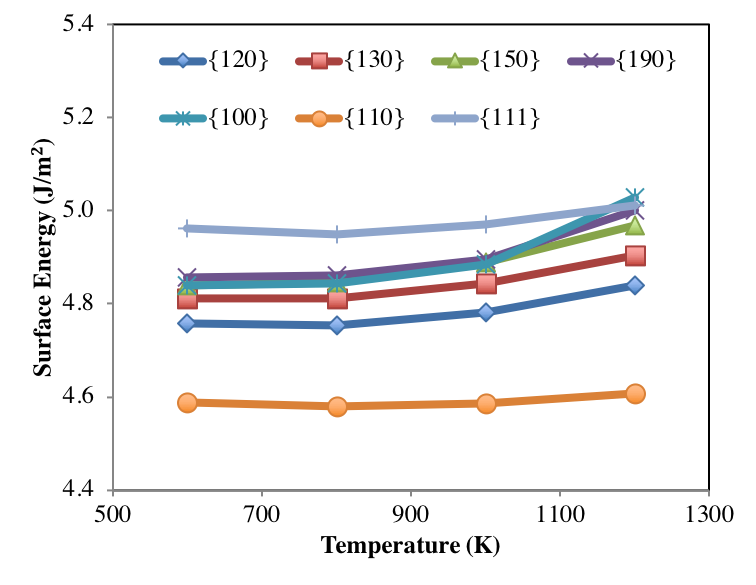
\includegraphics[width=0.6\textwidth]{mosurf.png}
 \caption{The bcc Mo surface energy as a function of temperature for five unique grain boundaries.}
 \label{fig:mosurf}
\end{figure}

\begin{table}[h]
\caption{The bcc Mo surface energy from 600 K to 1200 K for seven unique surface orientations. Units in J/m$^{2}$. } \label{tab:mosurf}
\begin{center}
\begin{tabular}{|c|c|c|c|c|}
	\hline
	Orientation & 600 K & 800 K & 1000 K & 1200 K \\
	 \hline
	 \{120\} & 4.76 & 4.75 & 4.78 & 4.84 \\
	 \{130\} & 4.81 & 4.81 & 4.84 & 4.90 \\
	 \{150\} & 4.84 & 4.85 & 4.89 & 4.97 \\
	 \{190\} & 4.86 & 4.86 & 4.90 & 5.00 \\
	 \{100\} & 4.84 & 4.84 & 4.88 & 5.03 \\
	 \{110\} & 4.59 & 4.58 & 4.59 & 4.61 \\
	 \{111\} & 4.96 & 4.95 & 4.97 & 5.01 \\	 
	 \hline
\end{tabular}
\end{center}
\label{default}
\end{table}

\FloatBarrier



\subsection{BCC U Interfacial Energies}
\subsubsection{BCC U Grain Boundary Energies}

The bcc U grain boundary energy as a function of misorientation angle at 1200 K is shown in Fig. \ref{fig:u1200}. Similar to Fig. \ref{fig:mo600}, ten unique symmetric grain boundaries are investigated. Grain boundary planes studied within this work are labeled. Data points are connected with straight lines as a mean to guide the eye. The most prominent minima exists at the \{120\} and \{130\} grain boundary planes, whereas the most prominent maxima occurs at \{350\}, similar to results from bcc Mo. There is no known experimental or computational data on the grain boundary energy in bcc U for comparison.

\begin{figure}[h]
 \centering
 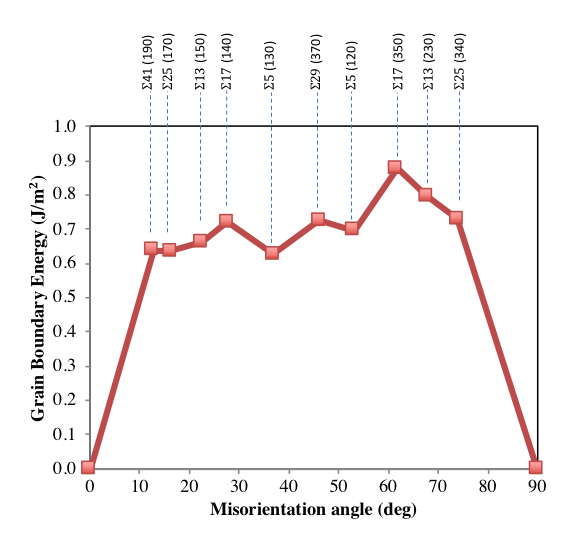
\includegraphics[width=0.6\textwidth]{u1200B.png} 
 \caption{The bcc U grain boundary energy as a function of misorientation angle at 1200 K.}
 \label{fig:u1200}
\end{figure}

The data from Fig. \ref{fig:u1200} is displayed in Table \ref{tab:u1200}, listing the ten unique symmetric tilt grain boundaries that were investigated for the bcc U system. The average standard deviation for each of these data points is 0.06 J/m$^{2}$. Excluding the low angle grain boundary of \{190\}, the minimum energy grain boundary plane examined is the \{130\}, while the maximum energy grain boundary plane examined is the \{350\}, with a difference between the maximum and minimum of 0.25 J/m$^{2}$. 

\begin{table}[h]
\caption{The bcc U grain boundary energy at 1200 K for ten unique symmetric tilt grain boundaries.} \label{tab:u1200}
\begin{center}
\begin{tabular}{|c|c|}
	\hline
	Grain Boundary Plane & Energy (J/m$^{2}$) \\
	 \hline
	 \{190\} & 0.64 \\
	 \{170\} & 0.64 \\
	 \{150\} & 0.66 \\
	 \{140\} & 0.72 \\
	 \{130\} & 0.63 \\	 
	 \{370\} & 0.73 \\
	 \{120\} & 0.70 \\
	 \{350\} & 0.88 \\
	 \{230\} & 0.80 \\
	 \{340\} & 0.73 \\
	 \hline
\end{tabular}
\end{center}
\label{default}
\end{table}

\FloatBarrier

The bcc U grain boundary energy as a function of temperature for four symmetric tilt grain boundaries and one asymmetric tilt grain boundary is shown in Fig. \ref{fig:utemp}. It can be observed that substantial variance is observed with increasing temperature for each respective grain boundary plane. There is a strong trend towards increasing grain boundary energy as a function of increasing temperature. The associated data is presented in Table \ref{tab:utemp}. Over the given temperature range, grain boundary energies are observed to vary by as much as 0.42 J/m$^{2}$. 

\begin{figure}[h]
 \centering
 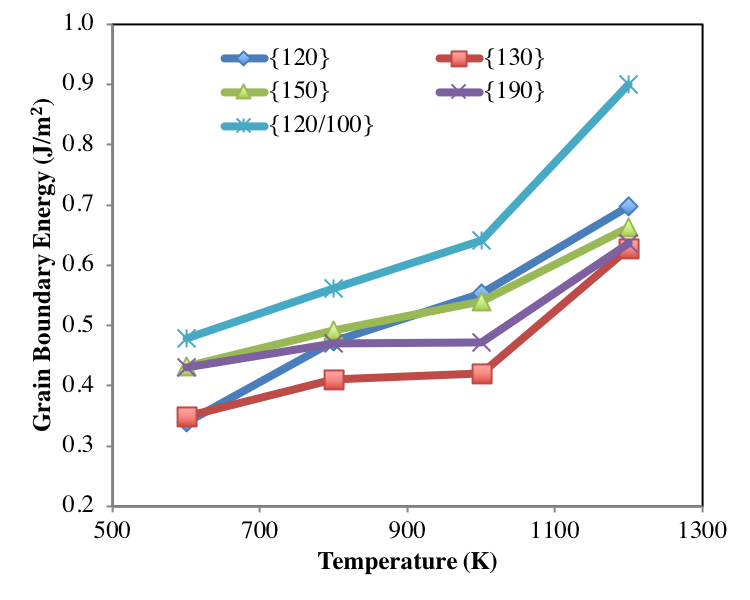
\includegraphics[width=0.6\textwidth]{u_temp.png} 
 \caption{The bcc U grain boundary energy as a function temperature for five unique grain boundaries.}
 \label{fig:utemp}
\end{figure}

\FloatBarrier

\begin{table}[h]
\caption{The bcc U grain boundary energy from 600 K to 1200 K for five unique grain boundaries. Units in J/m$^{2}$. } \label{tab:utemp}
\begin{center}
\begin{tabular}{|c|c|c|c|c|}
	\hline
	Grain Boundary Plane & 600 K & 800 K & 1000 K & 1200 K \\
	 \hline
	 \{120\} & 0.34 & 0.47 & 0.55 & 0.70 \\
	 \{130\} & 0.35 & 0.41 & 0.42 & 0.63 \\
	 \{150\} & 0.43 & 0.49 & 0.54 & 0.66 \\
	 \{190\} & 0.43 & 0.47 & 0.47 & 0.64 \\
	 \{120/100\} & 0.48 & 0.56 & 0.64 & 0.90 \\	 
	 \hline
\end{tabular}
\end{center}
\label{default}
\end{table}

\FloatBarrier


\subsubsection{BCC U Surface Energies}

The bcc U surface energy for seven unique surfaces as a function of temperature is shown in Fig. \ref{fig:usurf} and the associated data is presented in Table \ref{tab:usurf}. It is observed that the \{110\} surface is the lowest energy surface in bcc U. This matches the results from bcc Mo in Fig \ref{fig:mosurf} and makes intuitive sense, as has been discussed. There is no statistically significant unique high energy surface, as multiple surface orientations possess approximately the same surface energy. The surface energy shows an increase as a function of increasing temperature, similar to the trends of grain boundary energy as a function of temperature in Fig. \ref{fig:utemp}. Over the given temperature range, surface energies vary by a maximum of 0.32 J/m$^{2}$.

\begin{figure}[h]
 \centering
 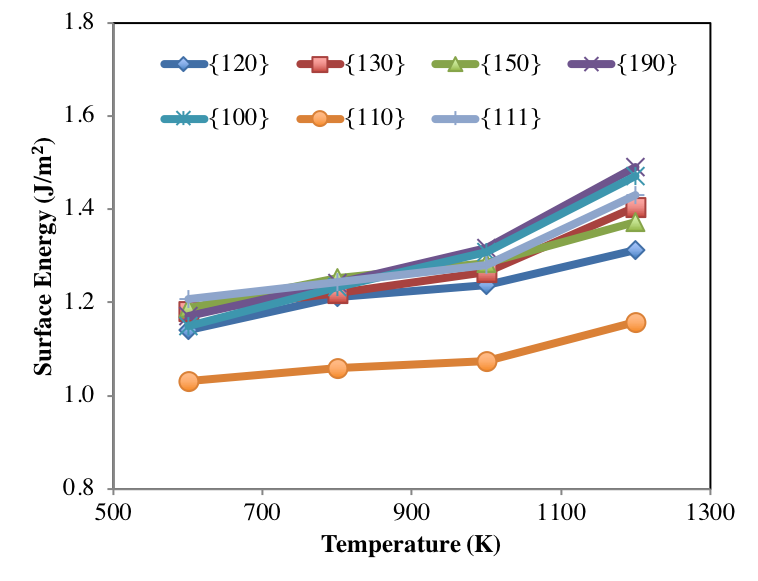
\includegraphics[width=0.6\textwidth]{usurf.png} 
 \caption{The bcc U surface energy as a function of temperature for seven unique surface orientations.}
 \label{fig:usurf}
\end{figure}

\begin{table}[h]
\caption{The bcc U surface energy from 600 K to 1200 K for seven unique surface orientations. Units in J/m$^{2}$. } \label{tab:usurf}
\begin{center}
\begin{tabular}{|c|c|c|c|c|}
	\hline
	Orientation & 600 K & 800 K & 1000 K & 1200 K \\
	 \hline
	 \{120\} & 1.14 & 1.21 & 1.24 & 1.31 \\
	 \{130\} & 1.18 & 1.22 & 1.27 & 1.41 \\
	 \{150\} & 1.19 & 1.25 & 1.29 & 1.37 \\
	 \{190\} & 1.17 & 1.24 & 1.32 & 1.49 \\
	 \{100\} & 1.15 & 1.23 & 1.31 & 1.47 \\
	 \{110\} & 1.03 & 1.06 & 1.07 & 1.16 \\
	 \{111\} & 1.21 & 1.24 & 1.28 & 1.43 \\	 
	 \hline
\end{tabular}
\end{center}
\label{default}
\end{table}

\FloatBarrier

\subsection{U-Mo Interfacial Energies}
\subsubsection{U-Mo Grain Boundary Energies}

The U-Mo grain boundary energy as a function of composition at 600 K is shown in Fig. \ref{fig:umo600} for four symmetric tilt grain boundaries and one asymmetric tilt grain boundary. It can be observed that there is a general trend of increasing grain boundary energy as a function of Mo concentration. This trend for each grain boundary plane is non-linear, but can be accurately fit with a second order polynomial. The data from Fig. \ref{fig:umo600} is displayed in Table \ref{tab:umo600}. All grain boundaries increase in energy by at least 1.2 J/m$^{2}$ progressing from bcc U to bcc Mo. Generally, the \{120\}, \{130\} or \{190\} grain boundary planes exhibit the lowest grain boundary energy, while the \{120/100\} asymmetric tilt grain boundary possesses the highest grain boundary energy. 

\begin{figure}[h]
 \centering
 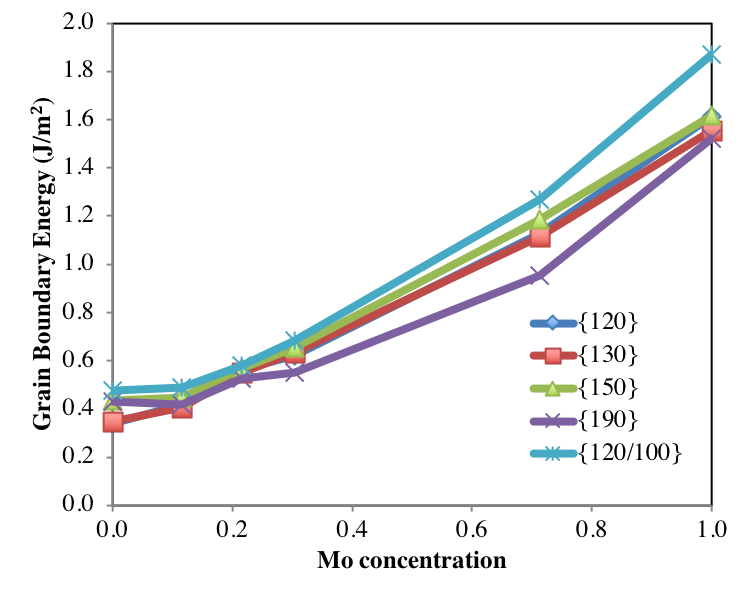
\includegraphics[width=0.6\textwidth]{uvsmo600.png} 
 \caption{The bcc U-Mo grain boundary energy as a function composition for five unique grain boundaries at 600 K. Mo concentration given in atomic fraction.}
 \label{fig:umo600}
\end{figure}

\FloatBarrier

\begin{table}[h]
\caption{The U-Mo grain boundary energy at 600 K for five unique grain boundaries. Units in J/m$^{2}$. } \label{tab:umo600}
\begin{center}
\begin{tabular}{|c|c|c|c|c|c|c|}
	\hline
 & U & U-5Mo & U-10Mo & U-15Mo & U-50Mo & Mo \\
\hline
\{120\} & 0.34 & 0.42 & 0.57 & 0.62 & 1.13 & 1.61 \\
\{130\} & 0.35 & 0.41 & 0.55 & 0.63 & 1.12 & 1.55 \\ 
\{150\} & 0.43 & 0.45 & 0.57 & 0.66 & 1.19 & 1.62 \\ 
\{190\}	 & 0.43 & 0.42 & 0.53 & 0.55 & 0.95 & 1.52 \\ 
\{120/100\} & 0.48 & 0.49 & 0.58 & 0.68 & 1.27 & 1.87 \\
 	 \hline
\end{tabular}
\end{center}
\label{default}
\end{table}

\FloatBarrier

The U-Mo grain boundary energy as a function of composition at 1200 K is shown in Fig. \ref{fig:umo1200} for four symmetric grain boundaries and one asymmetric grain boundary. The grain boundary energy shows a slight decrease, or possibly a plateau, with increasing Mo content up to approximately 30\% Mo content, after which the grain boundary energy increases with increasing Mo content. This trend for each grain boundary plane is non-linear, but can be accurately fit with a second order polynomial. The data from Fig. \ref{fig:umo1200} is displayed in Table \ref{tab:umo1200}. All grain boundary planes increase in energy by at least 0.93 J/m$^{2}$ progressing from bcc U to bcc Mo. Generally, the low-angle \{190\} grain boundary plane exhibits the lowest grain boundary energy, while the \{120/100\} asymmetric tilt grain boundary possesses the highest grain boundary energy.

\begin{figure}[h]
 \centering
 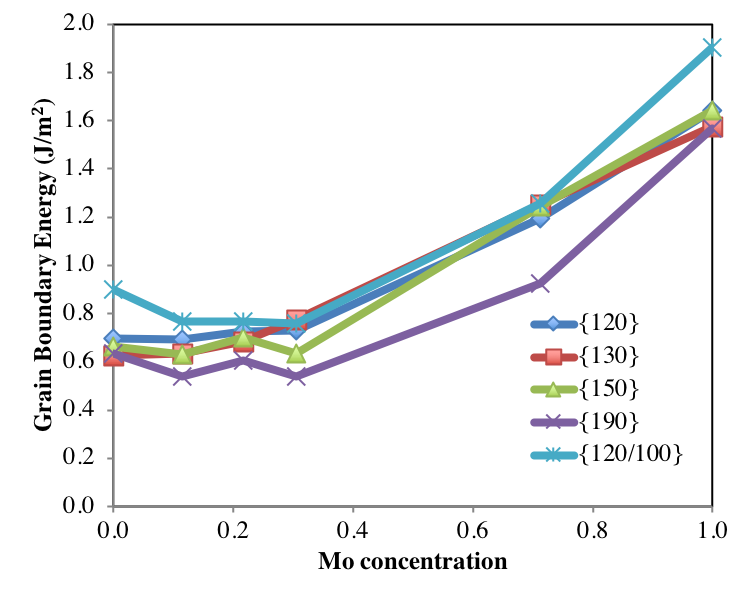
\includegraphics[width=0.6\textwidth]{uvsmo1200.png} 
 \caption{The bcc U-Mo grain boundary energy as a function composition for five unique grain boundaries at 1200 K. Mo concentration given in atomic fraction.}
 \label{fig:umo1200}
\end{figure}

\begin{table}[h]
\caption{The U-Mo grain boundary energy at 1200 K for five unique grain boundaries. Units in J/m$^{2}$. } \label{tab:umo1200}
\begin{center}
\begin{tabular}{|c|c|c|c|c|c|c|}
	\hline
 & U & U-5Mo & U-10Mo & U-15Mo & U-50Mo & Mo \\
\hline
\{120\}	 & 0.70 & 0.69 & 0.73 & 0.73 & 1.19 & 1.64 \\
\{130\}	 & 0.63 & 0.63 & 0.68 & 0.78 & 1.25 & 1.58 \\
\{150\}	 & 0.66 & 0.63 & 0.70 & 0.63 & 1.24 & 1.64 \\
\{190\}	 & 0.64 & 0.54 & 0.61 & 0.54 & 0.93 & 1.57 \\
\{120/100\} & 0.90 & 0.77 & 0.77 & 0.76 & 1.26 & 1.90 \\
 	 \hline
\end{tabular}
\end{center}
\label{default}
\end{table}

\FloatBarrier

To develop a more general picture of the grain boundary energy behavior as a function of composition and temperature, the results from the study of the five unique grain boundaries are averaged to create a single average grain boundary energy for a given composition and temperature. The results are shown in Fig. \ref{fig:avgvsmo}. The results show that for high Mo content (above approximately 30 atomic percent), grain boundary energy is relatively unchanged as a function of temperature. For low Mo content, the grain boundary energy increases with increasing temperature. This yields a grain boundary energy plateau region at 1200 K for Mo content less than 30 atomic percent. For temperatures below 1200 K, average grain boundary energy increases with increasing Mo content as well as increasing temperature. 

\begin{figure}[h]
 \centering
 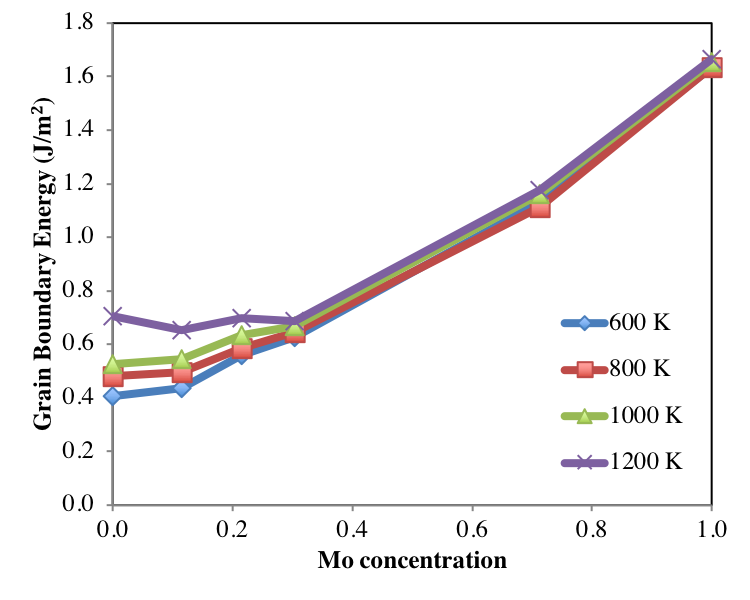
\includegraphics[width=0.6\textwidth]{avg_vs_mo.png} 
 \caption{The average bcc U-Mo grain boundary energy as a function composition and temperature. Mo concentration given in atomic fraction.}
 \label{fig:avgvsmo}
\end{figure}

\FloatBarrier

 
\subsubsection{BCC U-Mo Surface Energies}

The bcc U-Mo surface energy at 600 K for seven unique surface orientations as a function of composition is shown in Fig. \ref{fig:umosurf600} and the associated data is presented in Table \ref{tab:umosurf600}. It is observed that the \{110\} surface is the lowest energy surface in across the entire composition range. It can be observed that there is a general trend of increasing surface energy as a function of Mo concentration. This trend for each surface orientation is non-linear, but can be accurately fit with a second order polynomial. These trends match the trends of grain boundary energy as a function of temperature in Fig. \ref{fig:umo600}. All surface orientations increase in energy by at least 3.5 J/m$^{2}$ progressing from bcc U to bcc Mo. 

These results qualitatively agree with those of Mei, et al. \cite{zhigang2018}, who found the \{110\} surface to express the lowest energy for both bcc U and bcc Mo. Mei, et al. also found that surface energy increases with increasing Mo content. The absolute magnitude of the surface energy in this work does not closely correspond to the work of Mei, et al., as the bcc U surface energy in this work is lower than that of Mei, et al. (1.03 J/m$^{2}$ compared to 1.60 J/m$^{2}$) and the bcc Mo surface energy is much higher (4.59 J/m$^{2}$ compared to 2.89 J/m$^{2}$). It should be noted the simulations of Mei, et al. were conducted at 0 K. Given the qualitative agreement and the similar trend of surface energy as a function of Mo content, the results of both the first principles work of Mei, et al \cite{zhigang2018} and this molecular dynamics study are in correspondence.

\begin{figure}[h]
 \centering
 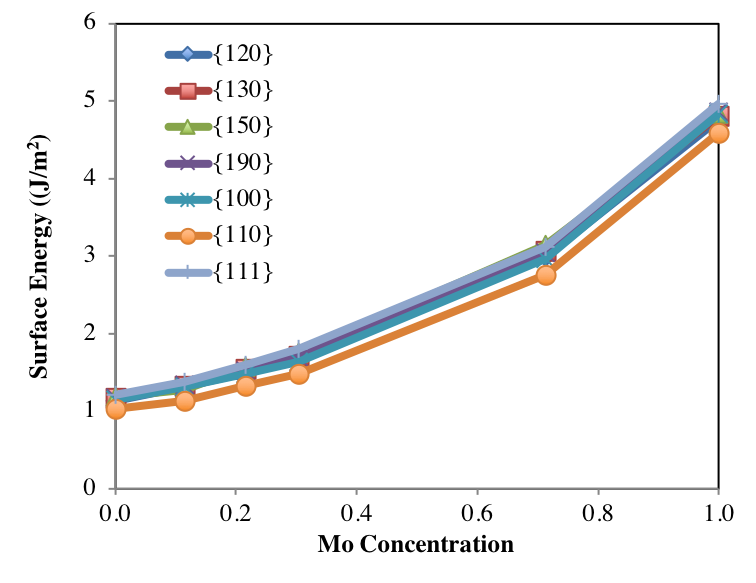
\includegraphics[width=0.6\textwidth]{umosurf600.png} 
 \caption{The bcc U-Mo surface energy at 600 K as a function of composition for seven unique surface orientations. Mo concentration given in atomic fraction.}
 \label{fig:umosurf600}
\end{figure}

\begin{table}[h]
\caption{The U-Mo surface energy at 600 K for seven unique surface orientations. Units in J/m$^{2}$. } \label{tab:umosurf600}
\begin{center}
\begin{tabular}{|c|c|c|c|c|c|c|}
	\hline
 & U & U-5Mo & U-10Mo & U-15Mo & U-50Mo & Mo \\
\hline
\{120\} & 1.14 & 1.31 & 1.50 & 1.69 & 2.99 & 4.76 \\
\{130\}	 & 1.18 & 1.33 & 1.55 & 1.72 & 3.07 & 4.81 \\ 
\{150\}	 & 1.19 & 1.28 & 1.57 & 1.76 & 3.14 & 4.84 \\
\{190\}	 & 1.17 & 1.34 & 1.52 & 1.70 & 3.05 & 4.86 \\
\{100\}	 & 1.15 & 1.31 & 1.48 & 1.63 & 2.96 & 4.84 \\
\{110\}	 & 1.03 & 1.13 & 1.33 & 1.48 & 2.75 & 4.59 \\
\{111\}	 & 1.21 & 1.38 & 1.60 & 1.80 & 3.12 & 4.96 \\
 	 \hline
\end{tabular}
\end{center}
\label{default}
\end{table}

\FloatBarrier

The bcc U-Mo surface energy at 1200 K for seven unique surface orientations as a function of composition is shown in Fig. \ref{fig:umosurf1200} and the associated data is presented in Table \ref{tab:umosurf1200}. The general trends as a function of composition are nearly identical to those at 600 K. The surface energy for all orientations monotonically increases as a second order polynomial with increasing Mo content and the \{110\} surface is consistently the lowest in energy. All surface orientations increase in energy by at least 3.4 J/m$^{2}$ progressing from bcc U to bcc Mo. 

\begin{figure}[h]
 \centering
 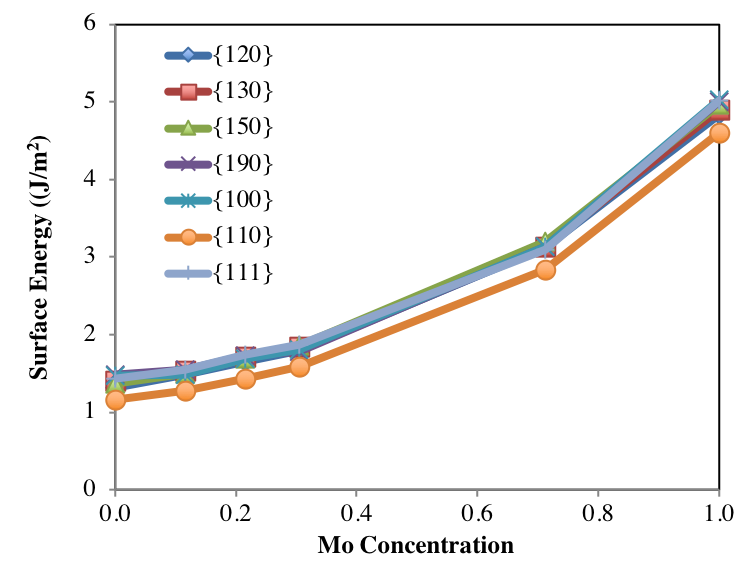
\includegraphics[width=0.6\textwidth]{umosurf1200.png} 
 \caption{The bcc U-Mo surface energy at 1200 K as a function of composition for seven unique surface orientations. Mo concentration given in atomic fraction.}
 \label{fig:umosurf1200}
\end{figure}

\begin{table}[h]
\caption{The U-Mo surface energy at 1200 K for seven unique surface orientations. Units in J/m$^{2}$.} \label{tab:umosurf1200}
\begin{center}
\begin{tabular}{|c|c|c|c|c|c|c|}
	\hline
 & U & U-5Mo & U-10Mo & U-15Mo & U-50Mo & Mo \\
\hline
\{120\} & 1.31 & 1.49 & 1.66 & 1.80 & 3.12 & 4.84 \\
\{130\}	 & 1.41 & 1.54 & 1.71 & 1.84 & 3.13 & 4.90 \\ 
\{150\}	 & 1.37 & 1.49 & 1.69 & 1.85 & 3.20 & 4.97 \\
\{190\}	 & 1.49 & 1.55 & 1.73 & 1.78 & 3.13 & 5.00 \\
\{100\}	 & 1.47 & 1.49 & 1.69 & 1.81 & 3.13 & 5.03 \\
\{110\}	 & 1.16 & 1.28 & 1.44 & 1.59 & 2.83 & 4.61 \\
\{111\}	 & 1.43 & 1.55 & 1.74 & 1.88 & 3.10 & 5.01 \\
 	 \hline
\end{tabular}
\end{center}
\label{default}
\end{table}

\FloatBarrier

To develop a more general picture of the surface energy behavior as a function of composition and temperature, the results from the study of the seven unique surface orientations are averaged to create a single average surface energy for a given composition and temperature. The results are shown in Fig. \ref{fig:avgvsmoS}. It is observed that there is a larger increase in surface energy as a function of temperature at low Mo content and very minimal variance as a function of temperature for high Mo content. Regardless of temperature, the surface energy increases with increasing Mo content. 

\begin{figure}[h]
 \centering
 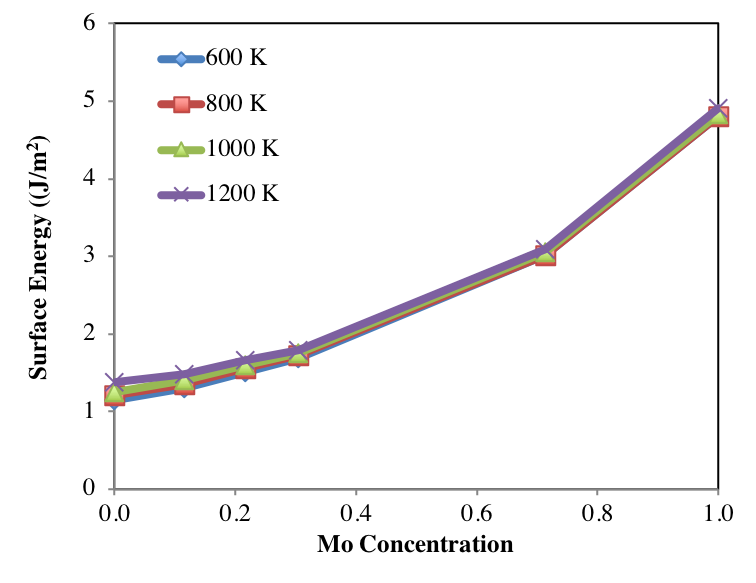
\includegraphics[width=0.6\textwidth]{umoavgsurf.png} 
 \caption{The average bcc U-Mo surface energy as a function composition and temperature for seven unique surface orientations. Mo concentration given in atomic fraction.}
 \label{fig:avgvsmoS}
\end{figure}

\FloatBarrier

\subsection{Discussion}

Given that the grain boundary formation energy is much lower in bcc U than in bcc Mo, it is much more energetically favorable for the U-10Mo to form bcc U grain boundaries, and subsequently deplete Mo at grain boundaries. Thus, the driving force for Mo depletion is the nature of the grain boundary energy for each of the pure bcc systems. This driving force is diminished with increasing temperature, but does not wholly dissipate. Regardless, it is suggested that the grain boundaries within U-Mo will not be totally devoid of Mo, as there are competing energetic factors. Depleting Mo from grain boundaries forces this Mo back into solution in bcc U-Mo, thus increasing the Mo content of the alloy. The formation energy of U-Mo is given by equation \ref{eqn:eform}

\begin{equation}
\label{eqn:eform}
E_{nf}= \frac{ E_{UMo} - E_{U} \times N_{U} - E_{Mo} \times N{Mo} }{ N_{U} + N_{Mo} }
\end{equation}

where E$_{UMo}$ is the energy of the alloy system, E$_{U}$ is the energy per atom of bcc U, N$_{U}$ is the number of U atoms in the alloy, E$_{Mo}$ is the energy per atom of bcc Mo and N$_{Mo}$ is the number of Mo atoms in the alloy. The formation energy of U-Mo increases with increasing Mo content in the U-rich region, as shown in Fig. \ref{fig:umoform}. Thus, by depleting Mo from grain boundaries in U-10Mo, the energy of the system is reduced, but there is an energetic penalty paid by increasing the Mo content of the bulk alloy, and thus the energy of the alloy (entropic contributions are neglected in this analysis). This energetic penalty should decrease with increasing grain size, as the depletion of Mo at grain boundaries would result in a progressively smaller increase of Mo concentration in the bulk as grain size increases. These competing mechanisms are both at work and determine how the atomistic configuration evolves, and the nature of the resulting Mo depletion at grain boundaries. Since the qualitative energetic trends also apply to surface energies, it is expected that Mo would deplete at surfaces as well. The result of this energetic competition can be elucidated by a hybrid Monte Carlo/Molecular Dynamics simulation, where both the depletion of Mo at grain boundaries and the subsequent increase in energy of the bulk are taken into consideration.

\begin{figure}[h]
 \centering
 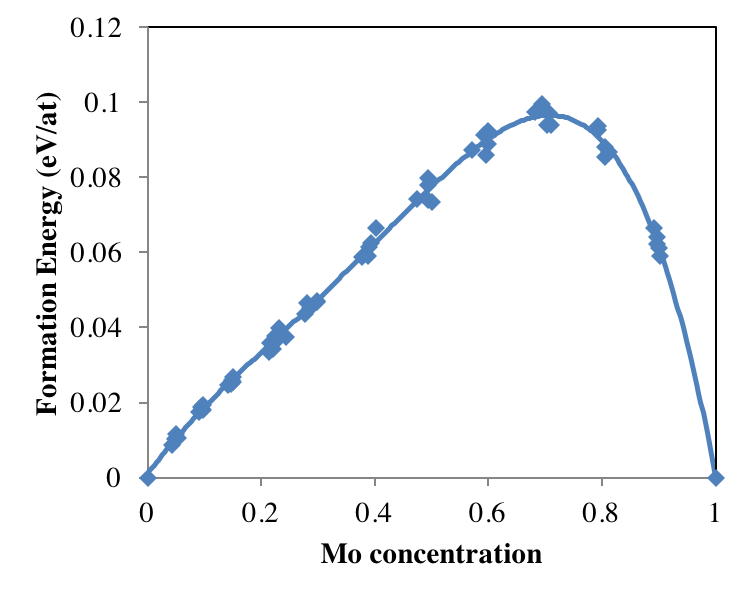
\includegraphics[width=0.6\textwidth]{umoform.png} 
 \caption{The formation energy of bcc U-Mo as a function of Mo concentration at 1000 K.}
 \label{fig:umoform}
\end{figure}

\subsection{Monte Carlo/Molecular Dynamics Mo depletion}
In order to further explore and verify the energetic properties of interfaces in U-Mo systems, a set of hybrid MC/MD simulations were performed on a \{120\} symmetric tilt grain boundary in U-10Mo. This type of simulation allows for substantial concentration movement that is essentially impossible to achieve in a strictly molecular dynamics simulation, where concentration movement is limited to point defect diffusion. As previously mentioned, this method can also account for the energetic preference of depleting Mo at grain boundaries and the energetic penalty of increasing the Mo content of the bulk. While free energy is not specifically investigated, the potential energy should act as the dominant driver of free energy within these systems. Individual simulations were performed at 600 K, 800 K, 1000 K and 1200 K to investigate the nature of Mo segregation and the degree to which the variation in energetic properties as a function of temperature results in variation in Mo segregation. 

An example system at 600 K is shown in Fig. \ref{fig:600mcmd}, where both the initial (top) and final (bottom) configurations are shown. Only Mo atoms are displayed within the supercell, for clarity. As the system is periodic, two grain boundaries are present within the system: at the simulation box edge, and in the center of the supercell (overlaid with a dashed red line). Throughout the simulation, atoms are swapped, and this results in a depletion of Mo at the grain boundaries. This is observed by an increase in empty space in Fig. \ref{fig:600mcmd} along the dashed red line and at either end of the simulation box. This apparent empty space is occupied by U atoms, which are not shown.

\begin{figure}[h]
 \centering
 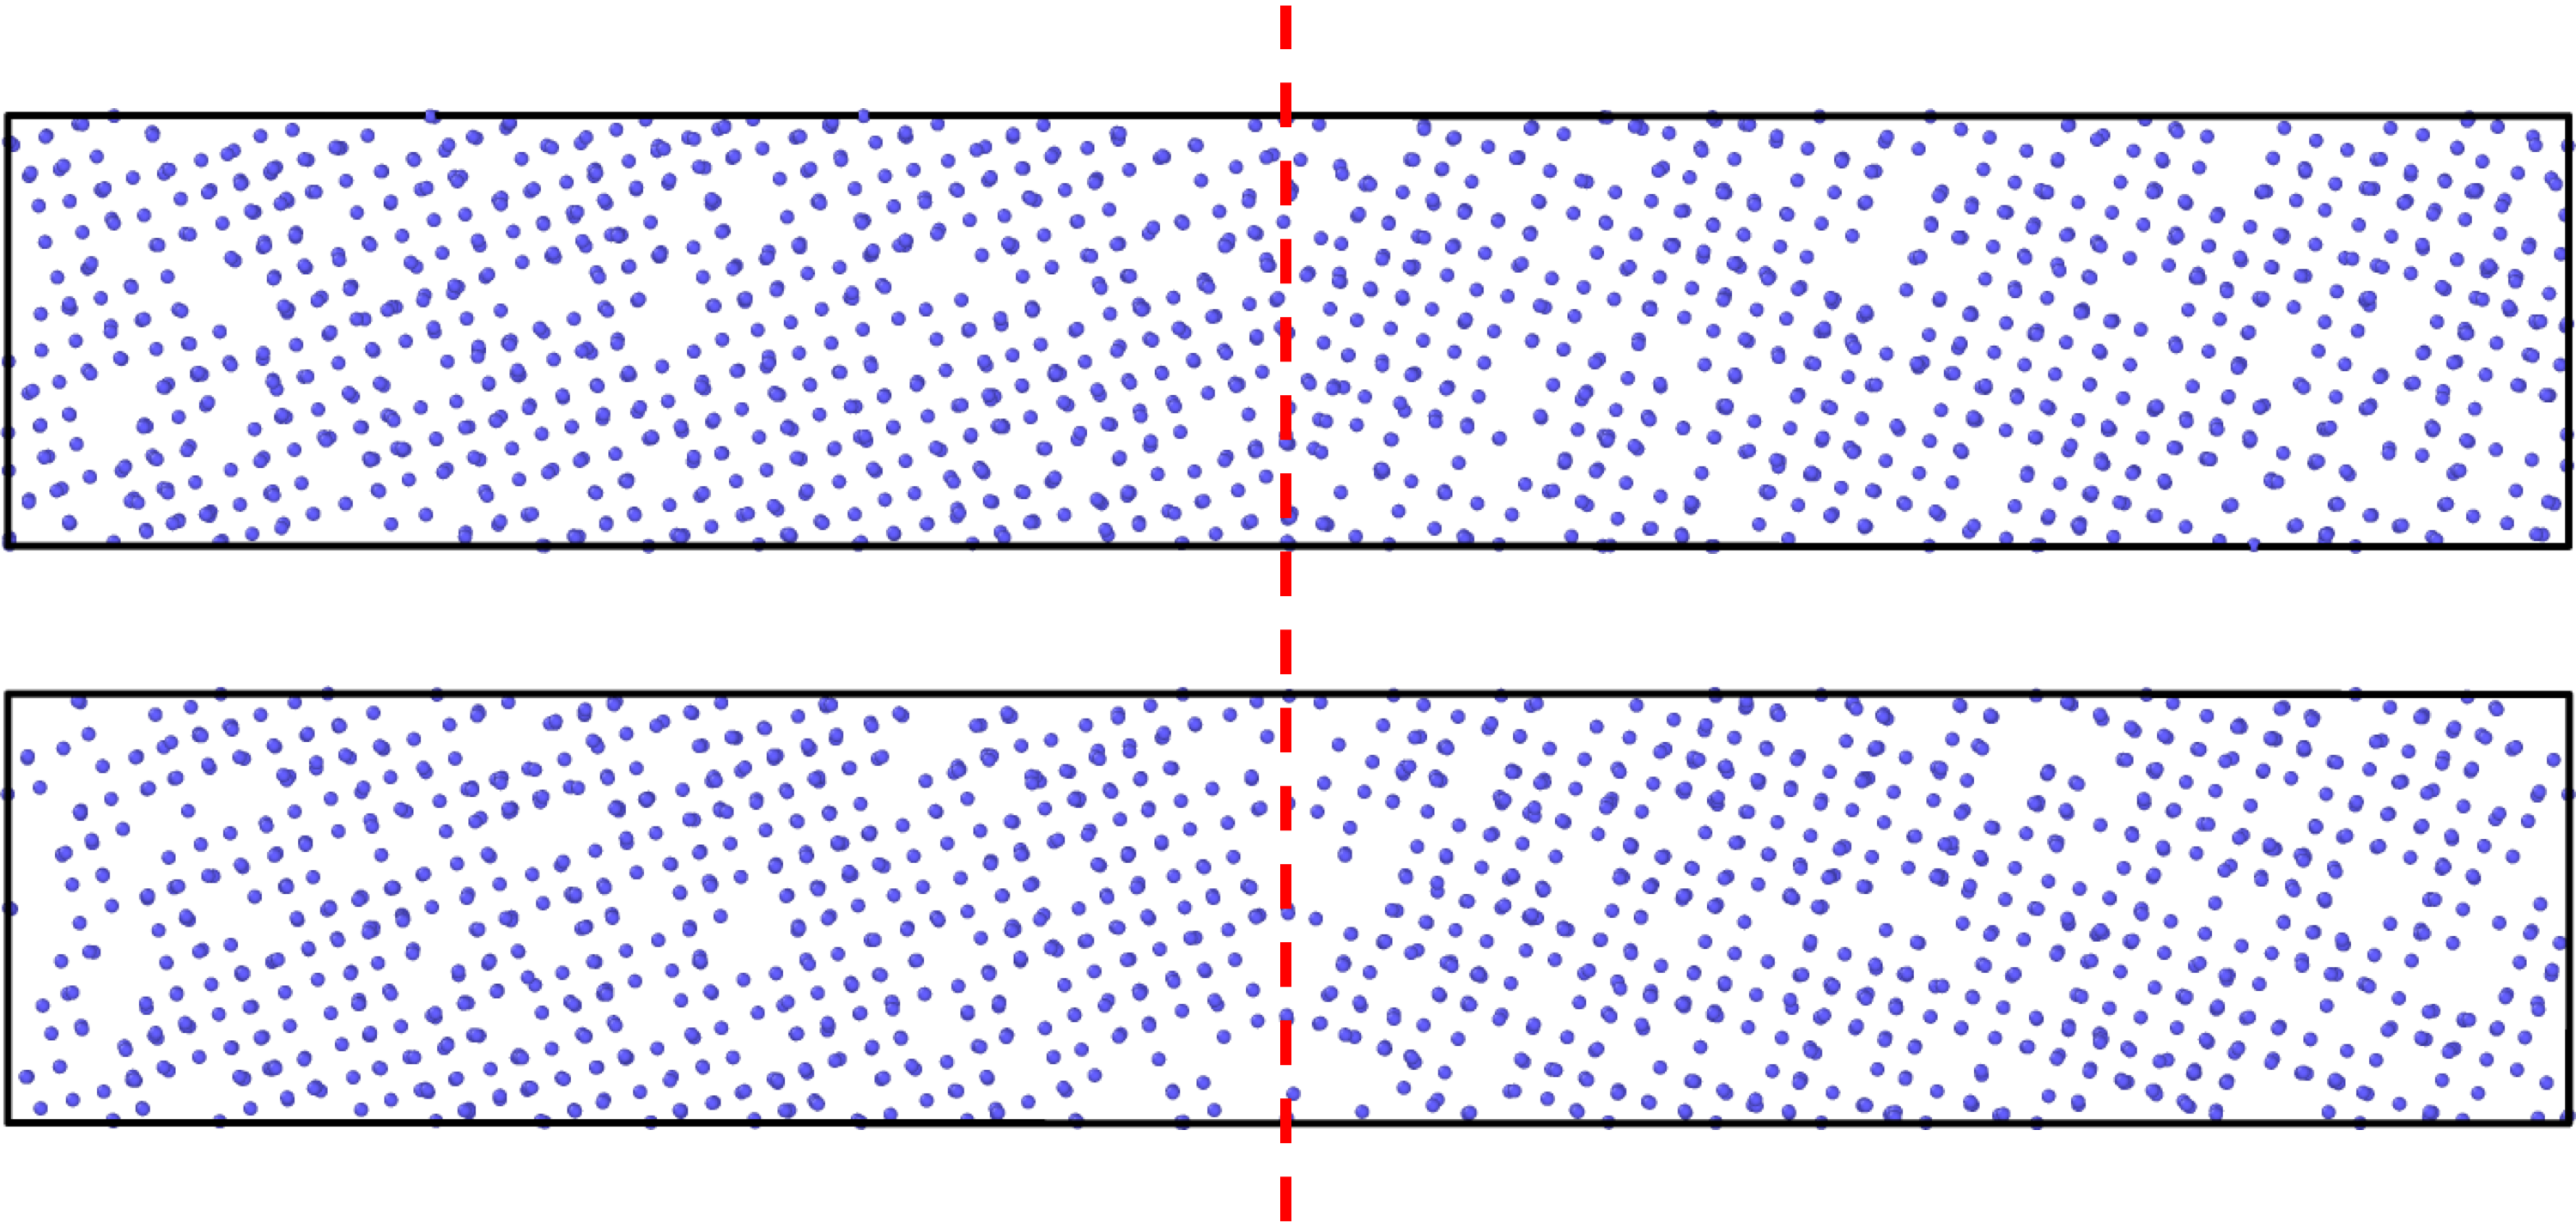
\includegraphics[width=0.8\textwidth]{600mcmd.png} 
 \caption{Mo atoms in a U-10Mo system with \{120\} symmetric tilt grain boundaries before and after the atom swapping simulation. The grain boundaries are at the center of the supercell (dashed red line) and at the ends of the simulation box with periodic boundaries. The top figure is initial distribution of Mo atoms, the bottom is the final distribution of Mo atoms.}
 \label{fig:600mcmd}
\end{figure}

\FloatBarrier

The amount of Mo segregation is quantified by dividing the supercell into 50 individual bins along the length of the supercell and counting the number of Mo atoms that reside within each bin and comparing the initial and final configurations. This is displayed in Fig. \ref{fig:600mcmdA}. The initial concentration profile is that of a random alloy, with an average of approximately 67 Mo atoms per bin and a standard deviation of 10 Mo atoms. In the final configuration, the standard deviation increased to 18 Mo atoms, while there is a statistically significant reduction in the number of Mo atoms at the grain boundaries, which occur at 0 and +/- 90 in the Y direction. There is a corresponding enrichment of Mo within the grains, as the concentration is conserved. By looking at the number of Mo atoms in the eight nearest bins to each of the grain boundaries (four bins on either side of each grain boundary), we can further quantify the reduction in the number of Mo atoms near the grain boundary. By combining the results for each grain boundary, there is a total reduction of 98 Mo atoms in the near-grain boundary region (527 atoms initially, 429 atoms at the end of the simulation). It can also be observed that there is not a total depletion of Mo at grain boundaries, as some Mo does still reside in the grain boundary regions. This corresponds with the previous discussion regarding the competing mechanisms of reducing Mo content at the grain boundary to reduce the energy of the grain boundary while increasing the energy of the bulk by increasing the Mo content in the bulk.

\begin{figure}[h]
 \centering
 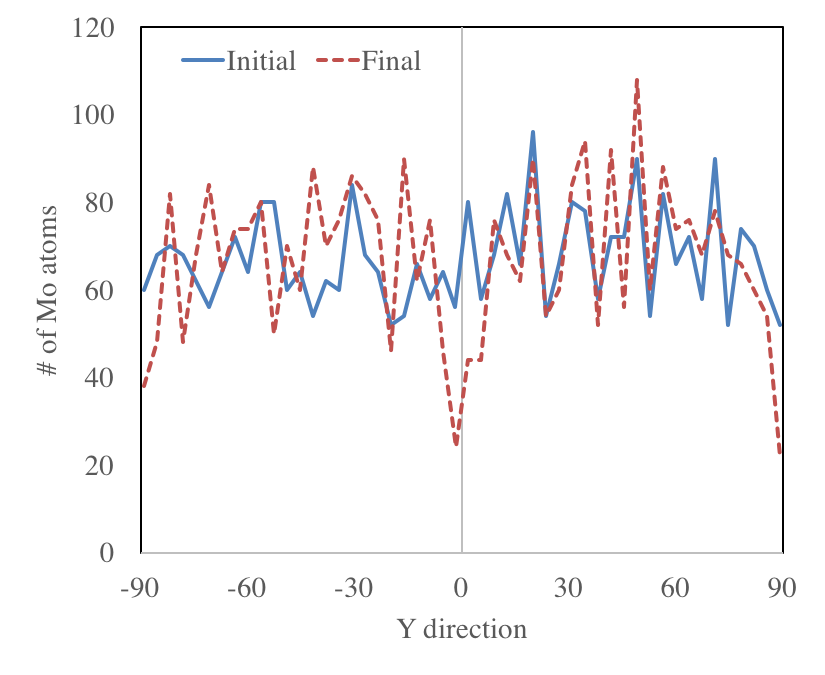
\includegraphics[width=0.6\textwidth]{600mcmdA.png} 
 \caption{Mo atoms with \{120\} symmetric tilt grain boundaries before and after the atom swapping simulation. The grain boundary is located at 0 and $\pm$90 in the y-direction. The blue solid line is the initial distribution of Mo atoms, and the red dashed line is final distribution of Mo atoms.}
 \label{fig:600mcmdA}
\end{figure}

\FloatBarrier

The number of Mo atoms as a function of position in the final state for simulations conducted at 600 K, 800 K, 1000 K and 1200 K are displayed in Fig. \ref{fig:mcmdtemp} and a summary of the number of Mo atoms near the grain boundary is displayed in Table \ref{tab:mcmdtemp}. It can be seen from both the table and the figure that there is depletion of Mo along the grain boundaries at all temperatures investigated. However, the degree to which the depletion of Mo occurs is reduced with increasing temperature. This is in agreement with the previous findings from Fig. \ref{fig:avgvsmo}. 
 
\begin{figure}[h]
 \centering
 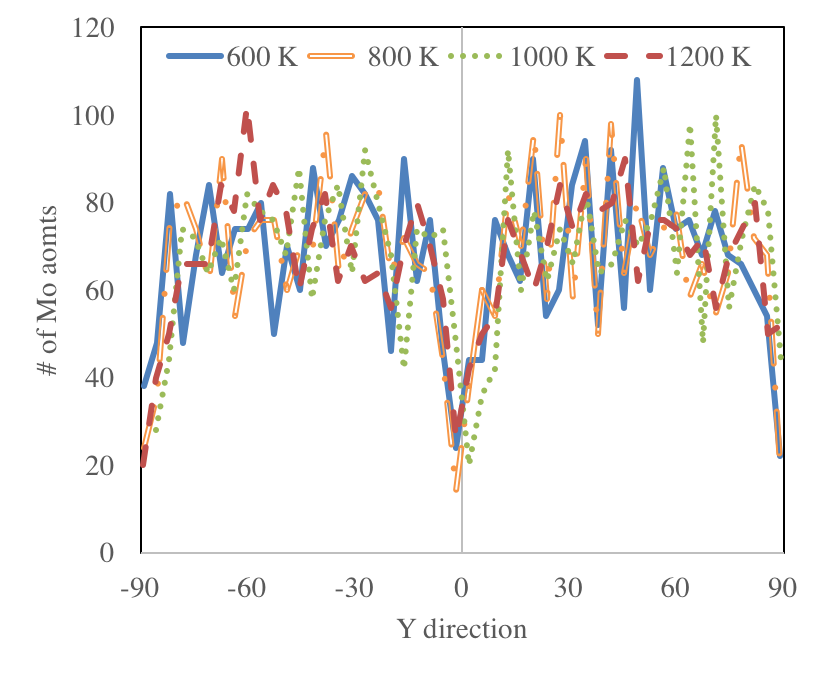
\includegraphics[width=0.6\textwidth]{mcmdtemp.png} 
 \caption{Mo atoms with \{120\} symmetric tilt grain boundaries after the atom swapping simulation at 600 K, 800 K, 1000 K and 1200 K. The grain boundary is located at 0 and $\pm$90 in the y-direction. The blue solid line is at 600 K, the hollow orange line is at 800 K, the green dotted line is at 1000 K and the red dashed line is at 1200 K.}
 \label{fig:mcmdtemp}
\end{figure}

\begin{table}[h]
\caption{The number of Mo atoms in the near-grain boundary region before and after the MC/MD simulation. } \label{tab:mcmdtemp}
\begin{center}
\begin{tabular}{|c|c|c|c|}
	\hline
Temperature & Initial & Final & Difference \\
\hline
600 K & 527 & 429 & 98 \\
800 K & 527 & 447 & 80\\ 
1000 K & 524 & 447 & 77 \\
1200 K & 523 & 444 & 79 \\
 	 \hline
\end{tabular}
\end{center}
\label{default}
\end{table}

\FloatBarrier

\section{Conclusions}

In this study, the grain boundary energy and surface energy for bcc U, bcc Mo and U-Mo alloys were calculated as a function of temperature and at various orientations. It is observed that bcc U and bcc Mo display similar grain boundary energy landscapes with respect to the $\langle$100$\rangle$ tilt axis, with the most prominent minima occurring at the \{130\} and \{120\} symmetric tilt grain boundary planes. In both systems, the \{110\} surface energy is the lowest in energy of all surfaces investigated. Grain boundary and surface energies of bcc Mo show minimal variation with increasing temperature while bcc U interfaces show a significant increase in energy with increasing temperature. The bcc Mo interfacial energies are substantially higher than those of bcc U. This is the driving force behind the phenomenon of Mo depletion at grain boundaries that has been observed in U-Mo fuels. The magnitude of the difference in interfacial energies between bcc Mo and bcc U decreases with increasing temperature. Grain boundaries in U-Mo are not expected to completely deplete Mo, as there is a competition between decreasing the energy of the grain boundary (by depleting Mo) and increasing the energy of the bulk (by subsequently increasing Mo content). Finally, active depletion of Mo at grain boundaries was performed via a series of hybrid MC/MD simulations. These simulations confirmed that the Mo concentration is reduced at grain boundaries, but that Mo is not fully depleted. These simulations also showed that the degree of Mo depletion is reduced as a function of increasing temperature. 

That the driving force behind Mo depletion at grain boundaries was uncovered is significant, but equally significant is the finding that this driving force is diminished at higher temperatures. Thus, fabrication processes such as high temperature annealing should inhibit Mo depletion along grain boundaries, resulting in a more homogeneous concentration of Mo, regardless of internal grain boundaries. The information within this manuscript can also be utilized by mesoscale models to simulate Mo depletion along grain boundaries and their subsequent deleterious effects on swelling of U-Mo fuel.

\section{Acknowledgement}
This work was supported by the U.S. Department of Energy, Office of Material Management and Minimization, National Nuclear Security Administration, under DOE-NE Idaho Operations Office Contract DE-AC07-05ID14517. This manuscript has been authored by Battelle Energy Alliance, LLC with the U.S. Department of Energy. The publisher, by accepting the article for publication, acknowledges that the U.S. Government retains a nonexclusive, paid-up, irrevocable, worldwide license to publish or reproduce the published form of this manuscript, or allow others to do so, for U.S. Government purposes. This research made use of the resources of the High Performance Computing Center at Idaho National Laboratory, which is supported by the Office of Nuclear Energy of the U.S. Department of Energy and the Nuclear Science User Facilities.

\bibliography{MARMOTbib}


\end{document} 
